% Chapter Template

\chapter{Puzzles} % Main chapter title

\label{sec:Puzzles} % Change X to a consecutive number; for referencing this chapter elsewhere, use \ref{ChapterX}
%----------------------------------------------------------------------------------------
%	SECTION 1
%----------------------------------------------------------------------------------------

\Section{Sliding Puzzle}


%-----------------------------------
%	SUBSECTION 1.1
%-----------------------------------
\Subsection{History - the 15-Puzzle}


The first puzzle I will focus on in this thesis is the sliding puzzle (see \cite{SlidingPuzzleWiki}) whose most common variant is the 15-puzzle, seemingly invented in the late 19th century by Noyes Chapman (see \cite{SlidingPuzzleWolfram}), who applied in 1880 for a patent on what was then called "Block Solitaire Puzzle". In 1879, a couple of interesting notes (\cite{Johnson1879}), published in the American Journal of Mathematics proved that exactly half of the $16!$ possible ways of setting up the 16 tiles on the board lead to solvable puzzles. A more modern proof can be found in \cite{Archer1999}.
\\
\\
Since then, several variations of the 15-puzzle have become popular, such as the 24-puzzle. A rather contrived but interesting one is the coiled 15-puzzle (\cite{Coiled15Puzzle}), where the bottom-right and the top-left compartments are adjacent; the additional move that this allows renders all $16!$ configurations solvable. 



\begin{figure}[H]
\centering
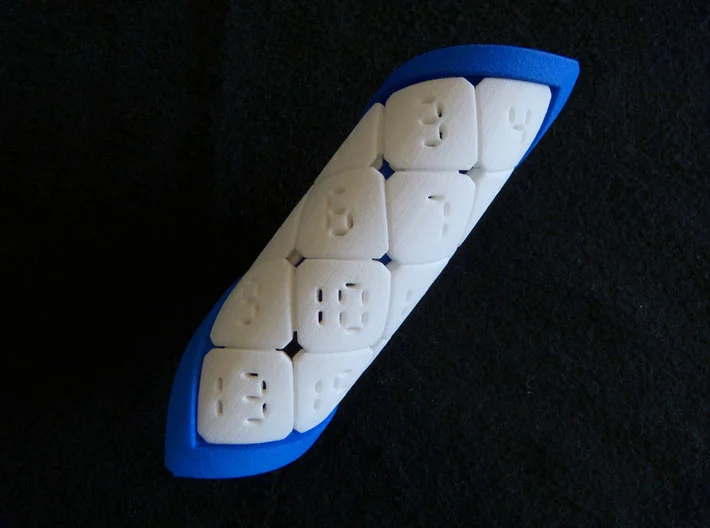
\includegraphics[scale=0.3]{./Figures/coiled15puzzle}
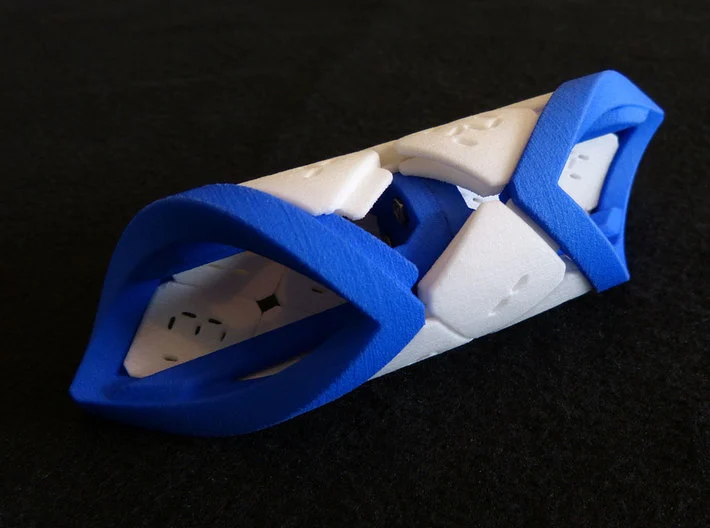
\includegraphics[scale=0.3]{./Figures/coiled15puzzle2.png}
\caption[Coiled 15-puzzle]{Coiled 15-puzzle}
\end{figure}


\noindent It is easy to see why this is the case, let me discuss why: given a configuration $c$ of the tiles, let us define the permutation $p(c)$ corresponding to enumerating the tiles row by row (top to bottom), left to right for odd rows and right to left for the even rows, ignoring the empty compartment. For the following left-hand-side15-puzzle $c_{l}$ we have $p(c_{l})$ = (1, 6, 2, 3, 4, 7, 10, 5, 9, 15, \red 14 \black, \blue 11, 8\black, 12, 13):

\begin{fifteen}
\setrow{4}{1,6,2,3}
\setrow{3}{5,10,7,4}
\setrow{2}{9,15,\red14\black,\blue11}
\setrow{1}{13,12,,\blue 8}
\end{fifteen}
% 
\begin{fifteen}
\setrow{4}{1,6,2,3}
\setrow{3}{5,10,7,4}
\setrow{2}{9,15,,\blue11}
\setrow{1}{13,12,\red14\black,\blue8}
\end{fifteen}
\\
The parity $p(c)$ of a configuration $c$ cannot change via a legal move. Indeed, p(c) is clearly invariant by lateral move of a tile, so its parity is invariant too. A vertical move of a tile will displace a number in $p(c)$ by an even number of positions right or left. For instance, moving tile 14 above in $c_{l}$  into the empty compartment below it results in a new configuration $c_{r}$ with $p(c_{r})$ = (1, 6, 2, 3, 4, 7, 10, 5, 9, 15, \blue11, 8\black, \red14\black, 12, 13), which is equivalent to moving 14 by 2 positions on the right. This obviously cannot change the parity since exactly 2 pairs of numbers are now in a different order, that is (14, 11) and (14, 8) now appear in the respective opposite orders as (11, 14) and (8, 14). This is the crux of the proof of the well-known necessary condition (even parity of p(c)) for a configuration c to be solvable (see part I of \cite{Johnson1879}). In the case of the coiled puzzle, we can solve all configurations of even parity, since all the legal moves of the normal puzzle are allowed. In addition, we can for instance transition between the following 2 configurations, which clearly have respectively even and odd parities:

\begin{fifteen}
\centering
\setrow{4}{\red1\black,2,3,4}
\setrow{3}{5,6,7,8}
\setrow{2}{9,10,11,12}
\setrow{1}{13,14,15,}
\end{fifteen}
%
\begin{fifteen}
\setrow{4}{,2,3,4}
\setrow{3}{5,6,7,8}
\setrow{2}{9,10,11,12}
\setrow{1}{13,14,15,\red1\black}
\end{fifteen}
\\
\\
Since it is possible to reach an odd parity configuration, we conclude by invoking symmetry arguments that we can solve all $16!$ configurations. 


%-----------------------------------
%	SUBSECTION 1.2
%-----------------------------------
\Subsection{Search Space \& Solvability}
\label{Theory:SPSSS}

In this thesis, as well as in the code base (\cite{FB}) I have written to do this project, we will consider the general case of a board with n columns and m rows, where $(n, m) \in {\mathbb{N}^{+}}^{2}$, forming $n * m$ compartments. $n * m - 1$ tiles, numbered 1 to $n * m - 1$ are placed in all the compartments but one (which is left empty), and we can slide a tile directly adjacent to the empty compartment into it. Notice from a programming and mathematical analysis perspective, it is often easier to equivalently think of the empty compartment being moved into (or swapped with) an adjacent tile. Starting from a given shuffling of the tiles on the board, our goal will be to execute moves until the are tiles in ascending order: left to right, top to bottom (in the usual western reading order), the empty tile being at the very bottom right.
\\
\\
Note that the case where either n or m is 1 is uninteresting since we can only solve the puzzle if the tiles are in order to start with. For instance, in the (n, 1) case, we can only solve n of the $\frac{n!}{2}$ possible configurations. We will therefore only consider the case where both n and m are strictly greater than 1.
\\
\\
As hinted in the previous section when discussing the coiled 15-puzzle, we can note that the parity argument used there implies that in general, out of the $(n * m)!$ possible permutations of all tiles, only half are attainable and solvable. This gives us a neat way to generate \textit{perfectly shuffled} puzzles, and we make use of this in the code. When comparing various algorithms in later sections, I will compare them on a same set of shuffled puzzles, where the shuffling is either done via a fixed number of random moves from goal position, or via what I call \textit{perfect shuffle}, which means I give equal probability to each attainable configuration of the tiles. A simple way to achieve this is therefore to start with one randomly selected among the $(n * m)!$ permutations, and then to verify that the parity of that permutation is the same as that of the goal (for the given choice of n and m), and simply swap the first two (non-empty) tiles if it is not.




%-----------------------------------
%	SUBSECTION 1.3
%-----------------------------------
\Subsection{Optimal Cost \& God's Number}

Let us fix n and m, integers strictly greater than 1 and call $\mathcal{C}_{(n, m)}$ the set of all $\frac{(n * m)!}{2}$ solvable configurations of the n by m sliding-puzzle. For any $c \in \mathcal{C}_{(n, m)}$ we define the optimal cost $\mathcal{O}(c)$ to be the minimum number of moves among all solutions for c. Finally we define $\mathcal{G}(n, m)$, God's number for the n by m puzzle as  $\mathcal{G}(n, m) = \max_{c \in \mathcal{C}_{(n, m)}} \mathcal{O}(c)$. Note that since $\frac{(n * m)!}{2}$ grows rather quickly with n and m, it is impossible to compute $\mathcal{G}$ except in rather trivial cases.
\\
\\
A favourite past time among computer scientists around the globe is therefore to search for more refined lower and upper bounds for $\mathcal{G}(n, m)$, for ever increasing values of n and m. For moderate n and m, we can solve optimally all possible configurations of the puzzle and compute exactly $\mathcal{G}(n, m)$  (using for instance $A^{*}$ and an admissible heuristic (recall \ref{GSH}, and we shall see modest examples of that in the results section later). For larger values of n and m (say 5 by 5), we do not know what the God number is. Usually, looking for a lower bound is done by \textit{guessing} hard configurations and computing their optimal path via an optimal search. Looking for upper bounds is done via smart decomposition of the puzzle into disjoint nested regions and for which we can compute an upper bound easily (either by combinatorial analysis or via exhaustive search). See for instance \cite{KarlemoOstergard} for an upper bound of 210 on $\mathcal{G}(5, 5)$.
\\
\\
A very poor lower bound can be always obtained by the following reasoning: each move can at best explore three new configurations (4 possible moves at best if the empty tile is not on a border of the board (less if it is): left, right, up, down but one of which is just going back to an already visited configuration). Therefore, after $p$ moves, we would span at best $\mathcal{S}(p) = \frac{3^{p+1} - 1}{2}$ configurations. A lower bound can thus be obtained for $\mathcal{G}(n, m)$ by computing the smallest integer $p$ for which $\mathcal{S}(p) \ge \frac{(n * m)!}{2}$


%-----------------------------------
%	SECTION 2
%-----------------------------------
\Section{Rubik's Cube}



\Subsection{History -- from Erno Rubik to speed cubing competitions}
The second puzzle I will focus on is the Rubik's Cube (\textbf{RC}), invented in 1974 by Erno Rubik, originally known as \textit{Magic Cube} (see \cite{RubiksWiki}). Since it was commercialised in 1980, it has known a worldwide success: countless people are playing with the original 3x3x3 cube, as well as with variants of it of all shapes and sizes. Competitions bring together \textit{speedcubers} who have trained for years and memorized algorithms to solve the Rubik's in astonishingly fast times (seconds for the best ones). Some of the principles used by speedcubers generalise to different dimensions. As an example, it is quite impressive to watch \textit{Cubastic} solve a 15x15x15 cube in (only) two and a half hours! (see \cite{151515Rubiks}). The key insight to solving high dimensional \textbf{RC}s (short obviously of coming up with specific strategies) is the following: if we manage to group all the inside (i.e. not located on a corner or an edge) cubies by colour, and then all the non-corner edges on a given tranche of a face by colour, we are essentially reducing the cube to a 3x3x3, since no face rotation will ever undo these groupings. The picture below (\ref{fig:4442333}) shows my own 4x4x4 and 3x3x3 cubes arranged to be in identical configurations.
\begin{figure}[H]
  \noindent
  \makebox[\textwidth]{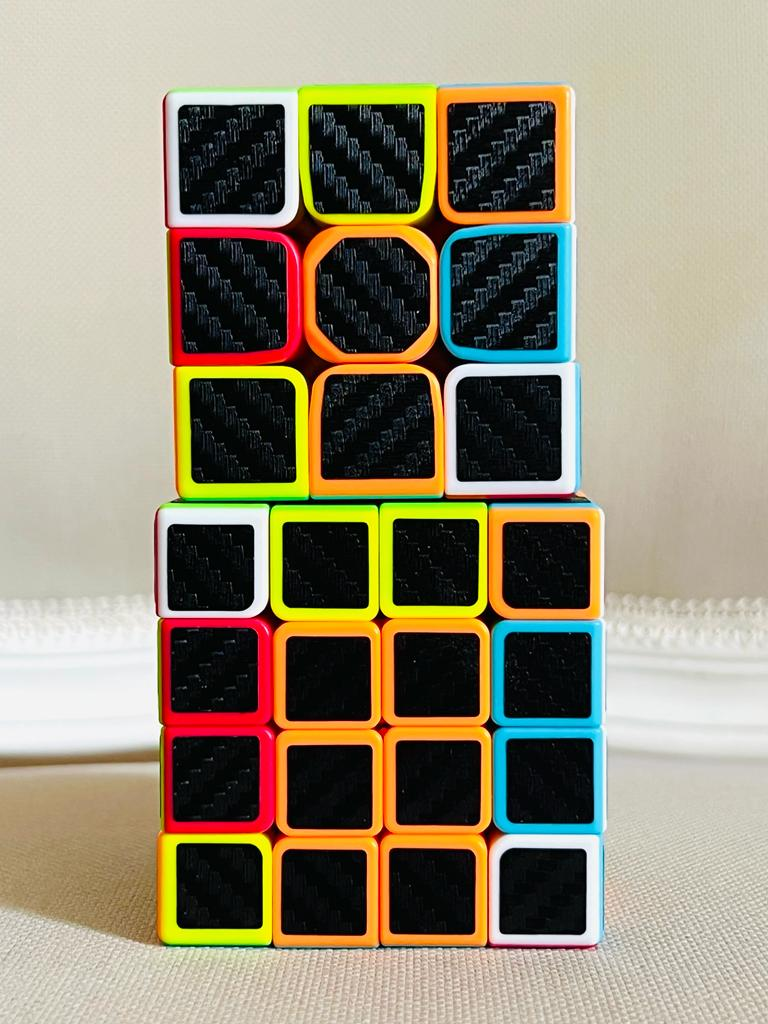
\includegraphics[scale=0.25]{./Figures/RC333444}}
  \caption[Reducing RC]{Reducing a 4x4x4 \textbf{RC} to a 3x3x3 -- home-made picture}
  \label{fig:4442333}
\end{figure}
\noindent If we can bring the 4x4x4 cube to such a configuration on all faces (which is not very hard), and if we know how to solve a 3x3x3, we are essentially done. (The additional degrees of freedom on the 4x4x4 complicate slightly the story since certain arrangements of colors which are possible on the 4x4x4 are not on the 3x3x3, e.g. red and white on opposite faces). Overall, the difficulty of hand-solving cubes does not grow as much with dimensionality as one would think, and the time difference comes mostly from the difficulty of handling and manipulating larger cubes.




\Subsection{Conventions: faces, moves and configurations}
I follow the conventions and notations of the \textbf{RC} community and refer to the faces as F (front), B (back), U (up), D (down), L (left) and R (right). It is common in \textbf{RC} jargon to refer to moves  by the name of the face that is rotated clockwise (when facing it), and by adding a \textit{'} for counter-clockwise rotations. Sometimes numbers are used to indicate repeated moves, though I will count that as multiple moves, since obviously e.g. U2 = U U = U' U'. As another example: F B' F2 means rotating the front face clockwise, the back face counter-clockwise, followed by the front face twice. The convention I follow is called the \textit{quarter-turn-metric}, and obviously the length of solutions is affected by which metric we use.
\\
Since I am interested in experimenting with \textit{no-human-knowledge} methods such as \textbf{DRL} and \textbf{DQL}, I will consider cubes which are identical up to full cube rotation such as the \textit{flattened} cubes on figure \ref{fig:configurations} to be different. They will be represented by different tensors in my code, and this is up to the solvers to make sense of things.

\begin{figure}[H]
  \noindent
  \makebox[\textwidth]{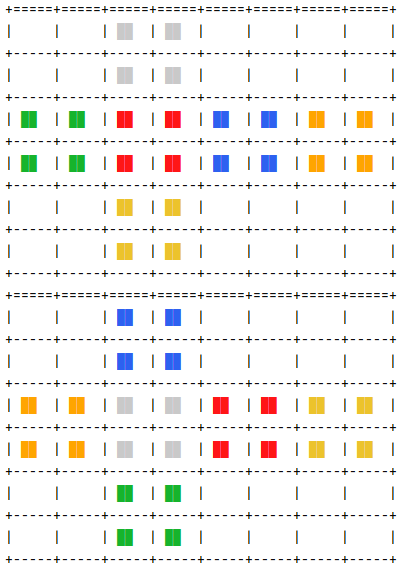
\includegraphics[scale=0.4]{./Figures/equivalentcubes}}
  \caption[Reducing RC]{Two equivalent configurations by full-cube-rotation}
  \label{fig:configurations}
\end{figure}

\noindent The \textbf{RC} has, as one would expect, an extremely large state space. I will compute the state space size for the 3x3x3 and 2x2x2 cubes in the next two subsections and discuss conditions under which a cube is solvable.

\Subsection{3x3x3 Rubik's -- search space, solvability \& God's number}
\label{Theory:333RCSSS}

A good strategy to compute the state space size of a the Rubik's of a given dimension is to compute:
\begin{itemize}
\item $N$: the number of possible arrangements of the \textit{cubies} (individual small cubes that constitute the Rubik's) in space, taking into account physical constraints and some invariants.
\item $D$: the number of possible configurations which are equivalent via full cube rotation in space.
\end{itemize}
The state space can then be considered to be either $\frac{N}{D}$ or $N$, depending on our representation (as mentioned earlier my code will treat each rotation of the cube in space as a different representation, so I shall not be dividing by $D$ below).

In order to compute $D$, we just need to realise that each configuration can be arranged in (only) 24 different ways via full cube rotation in space. In particular that means that there are 24 possible goal states (and not 6! as we might naively think at first), so for instance in figure \ref{fig:configurations} I could only have picked 2 out of 24 different configurations. Why is this? 
\\
Any of the six colors can be placed on the F face, and then any of the four adjacent colors can be placed on the U face (say). Once these two colors are chosen, the remaining faces are determined. This is not immediately obvious, but not difficult to convince oneself that this is the case with the following two observations about the structure of corner \textit{cubies}: first observation is that they have 3 determined colors, which are fixed once and for all. In particular, the fact that there is no corner with colors F and B, means that once the cube is in solved state, we have to have colors F and B on opposite faces, and similarly for colors U and D as well as colors L and R. Hence, having fixed the color on face F, the color on face B is fixed too. The second observation is that when facing a corner cubie, the order of its three color (e.g. enumerated clockwise) is invariant. For instance, consider the corner cubie with colors (F, R, U). No scrambling of the cube will ever produce clockwise order of e.g. (F, U, R). This is obvious once you consider that there is no move of the Rubik's cube you could not perform while holding a given corner fixed in space (e.g. by pinching that corner cubie with your fingers and never letting go of it).
\\
\\
Computing $N$ is a bit tricker. For the 3x3x3 Rubik's, each of the 8 corner cubies could be placed at one of the physical corner locations and oriented three different ways (rather than six, since as discussed earlier, the clockwise orientation of a given corner cubie can never be changed). We have therefore $8! . 3^{8}$ corner arrangements. Similarly, the 12 edge cubies can be placed at 12 physical edge locations and oriented 2 different ways, so we have another multiplicative factor of $12! . 2^{12}$. There are however some well-known parities (see \cite{Schoenert} for details) which are invariant under legal moves of the Rubik's cube and which reduce the number of arrangements that are physically attainable via face rotations. The \textit{corner orientation parity} (\textbf{COP}) for instance sums over the corner cubies the number of 120$^{o}$ rotations it would take to bring a given cubie to its standard orientation (i.e. compared to the top cube in figure \ref{fig:configurations}). It is easy to observe that the \textbf{COP} is invariant (\% 3) since any face rotation will displace four corner cubies, two of which see their individual \textbf{COP} increase by 2, and the other two by 1 (so a total increase of 6). Similarly, there are two additional parities called \textit{edge orientation parity} (\textbf{EOP}) and \textit{total permutation parity} (\textbf{TPP}) which are both invariant (\% 2) under face rotation. Overall, these three parities mean that only $1/12$ of the $8! . 3^{8} . 12! . 2^{12}$ arrangements are physically attainable, leaving us with a grand total of $43,252,003,274,489,856,000$ different cubes (still a rather staggeringly large number!).
\\
\\
Finally, let me mention that there is a long history of research into finding tighter and tighter bounds on the 3x3x3 God's number (usually, proofs of upper bounds were obtained and refined by decomposing the Rubik's moves group into subgroups, then finding upper bounds of distance between two elements of a given subgroup, and finally summing these upper bounds over the different subgroups). See e.g. \cite{RubiksChicago} for an exposition of this type of approach. In 2007, an upper bound of 34 in the quarter turn metric was published (\cite{RubiksRadu}) but the question got properly settled in \cite{RubiksGodNumber} by Google's researchers which used clever symmetry arguments to reduce the search space to the maximum, followed by Google's vast computing power capabilities to brute force solve all of the configurations they were left with. They concluded that the 3x3x3 Rubik's God number is in fact a mere 26.


\Subsection{2x2x2 Rubik's -- search space, solvability}
\label{Theory:222RCSSS}

For the 2x2x2 cube, there are eight possible ways of choosing the physical position of the eight corner cubies (and since there are known algorithms, such as R’ U R’ D2 R U’ R’ D2 R2, to swap exactly two and only two adjacent corners we know all can indeed be obtained). Each corner cubie can be oriented in 3 different ways, so we get a total of $8! . 3^{8}$ configurations. However, due to the \textbf{COP} parity discussed in the previous section, we conclude that only one third of these are attainable (namely those for which the \textbf{COP} is equal to 0 \% 3). Overall, this gives $8! * 3^{7}$ = 88,179,840 possible configurations (probably a larger number than most people would expect for a mere 2x2x2 cube).
\\
The insight and knowledge of this section has been useful for me to implement \textit{perfect scrambling} for the 2x2x2 \textbf{RC}. Indeed, the way I generate perfectly shuffled cubes is by randomly placing the 8 corners, then randomly choosing the orientation of the first 7, and finally fixing the $8^{th}$ corner's orientation to make sure COP is equal to 0 \% 3.
\\
Some quick googling suggests the 2x2x2 Rubik's God number to be 11 in the quarter turn metric, but I could not find any clear and definitive paper on this.


\Subsection{Rubik's -- multi-stage search}
\label{Theory:RCMSS}
Modern Rubik's domain-specific solvers (such as the Kociemba solver which I have used in this project as a comparison point) make use of a multi-stage search approach. Essentially, they just do what speedcubers do by hand, just much faster and better. The general idea is as follows: let us suppose we have a puzzle with a state space $\mathcal{S}$ of size $N$ (some large number) and one goal state $g$. Now imagine that we have discovered a much smaller subset of configurations $\mathcal{S}_{1} \in \mathcal{S}$ (say of size $n \ll N$) such that $g \in \mathcal{S}_{1}$ and such that it is \textit{easy} to check whether or not a given configuration $p \in \mathcal{S}$ belongs to $\mathcal{S}_{1}$. In addition, suppose we also have discovered a set of algorithms $\mathcal{A}_{1}$ (sequence of actions) under which elements of $\mathcal{S}_{1}$ are stable and which spans $\mathcal{S}_{1}$. Finally, suppose that we have a set of algorithms $\mathcal{A}_{2}$ which allow us to (provably) take any given configuration $p \in \mathcal{S}$ into $\mathcal{S}_{1}$ in a bounded number of steps. A viable strategy to solve any puzzle then becomes:
\begin{titlemize}{Multi-stage search}
\item If $p \in \mathcal{S}_{1}$, set $a_{2}$ to be the identity move in $\mathcal{S}$, and jump to step 3.
\item Apply a search algorithm (e.g. A$^{*}$ - or some variant such as IDA$^{*}$ (\cite{IDAWiki}) - restricting eligible actions to $\mathcal{A}_{2}$, until we find a sequence of actions $a_{2}$ such that $a_{2}(p) \in \mathcal{S}_{1}$
\item Apply our search algorithm to $a_{2}(p)$, restricting eligible actions to $\mathcal{A}_{1}$, until we find a sequence of actions $a_{1}$ such that $a_{1}(a_{2}(p)) = g$.
\item $a_{1} \circ a_{2}$ is our multi-stage solution
\end{titlemize}
Notice that this is exactly how beginners and advanced speedcubers solve the Rubik's cube, except they usually have more than 2 stages as described above. $S_{1}$ might for instance be the set of cubes where both lower layers are solved, the cross on the top layer as well as all corners are in their respective places (but maybe not oriented as expected), and then they search within a well-known and small set of algorithms how to get to the goal state. A previous stage might consist in $S_{2}$, the set of configurations where the two layers are solved, but the top layer is random, and then they will search for a sequence of moves to get into $S_{1}$, etc \dots


%-----------------------------------
%	SECTION 3
%-----------------------------------
\Section{Solving puzzles without human knowledge}
\label{sec:WHK}

In the upcoming implementation (\ref{sec:Implementation}) and results (\ref{sec:ResultsSP}, \ref{sec:ResRubiks}) sections, I will be discussing various solvers. I would put them broadly in four different categories, by decreasing level of human knowledge that has been assumed and handcrafted in them. Notice that my human-knowledge-required scale is obviously somewhat arbitrary, but good to keep in mind in later (and in particular results) sections.

\paragraph{Domain-specific solvers}
At 4 on the human-knowledge-required scale, I would put my NaiveSolver (handcrafted to solve the \textbf{SP}) as well as the hkociemba (2x2x2) and kociemba (3x3x3) open source implementations which I have integrated in my KociembaSolver. They make heavy use of specific knowledge about the two puzzles (see \ref{Theory:RCMSS}), not only about their mechanics, but also about how to actually (and provably) solve them.


\paragraph{Domain-specific heuristics}
At 3 on the human-knowledge-required scale, I put A$^{*}$-with-handcrafted-heuristics (e.g. Manhattan heuristic for the \textbf{SP}) algorithms. Constructing the heuristics usually require some knowledge about the puzzle's mechanics, but not necessarily about how to solve them efficiently (though of course knowing the latter might help come up with more efficient heuristics).


\paragraph{Supervised learning}
At 2 on the human-knowledge-required scale, I put my DeepLearner solver (also using A$^{*}$ but whose heuristic is learnt via \textbf{DL}). This solver does not require any knowledge of the structure or mechanics of the puzzle, nor of how to solve them, but just need a teacher algorithm to learn/extrapolate from.


\paragraph{Blind search\& unsupervised learning}
Finally at 1 on the human-knowledge-required scale, I put the blind solvers such as \textbf{BFS} and \textbf{DFS}. Also in that group I put A$^{*}$ with heuristics learnt using my DeepReinforcementLearner and DeepQLearner, and my MonteCarloSearchTree which all know (almost) nothing about the puzzles and do totally work from generic interfaces alone (states, transitions, etc \dots) and are operating in an unsupervised way.
\\
\\
One important comment I would make to end this section is that it is easy to inject, without realising or acknowledging it, specific knowledge into the solvers, or in the tensor representation of the puzzles that the solvers take as input. Pretty much all the papers about \textbf{RC} that I have surveyed chose a more compact representation for the cube than I have. They remove the centre cubies of the 3x3x3 cube since, they argue, those never move via face-turns. Some of them go much further and make use of various symmetry arguments to reduce the search space and reduce the \textbf{RC} to having one goal state (instead of 24). One of the main papers I have taken inspiration from for this project, \cite{DBLP:journals/corr/abs-1805-07470}, reduces the representation of the Rubik's considerably more, by making use of arguments about the physical structure of the edge and corner cubies: knowing the color of one of their face allows you do deduct the other faces, and therefore, they only need to track one face. I of course understand that they do that for the sake of reducing the size of the tensors representing the cube, and in order to remove redundant information. This is still \textit{cheating} a bit in my opinion, especially if you are claiming to solve these puzzles \textit{without-human-knowledge}, as we can only perform these dimensionality reduction tricks if we have external world knowledge about the physical structure of the puzzles. In this project, I have chosen as pure an approach as I could, and not only did not reduce the dimensionality of the tensor representation of the puzzles, but also, specifically for the Rubik's cube, I did not make use of invariance by spatial rotation of the full cube.



































